\chapter{Introduction to Pointer}
\section{Overview on Pointer}
If you already have sufficient understanding about Pointer in both C\# and C languages, you can skip this chapter. This chapter is for introducing beginners to the concept of pointer.

A pointer is essentially an address to an area of memory. You can represent what that pointer is supposed to be such as a pointer of integer, struct, classes, function or even another pointer.
To read and write memory that pointer is pointing to, you have to first dereference that pointer and you can do so by using asterisk in front of a pointer variable to dereference it, not to be confused with multiplication operator.

\lstinputlisting[style=customc, language=C]{codes/Chap3/Chap3Snippet1.c}
\newpage
The C snippet above first allocate with malloc function a new buffer of memory up to a size of int32\_t datatype and return a void* pointer which then get casted into int32\_t* pointer type. You can access the pointer in two ways, writing it similar fashion as you would when accessing an array and to use '*' operator to dereference the pointer to read and write the first datatype the pointer is currently pointing to.

Let's get started by creating a new "ChapterThree" directory and create a new file, "ChapThree.c" and open with your favorite editor.

We will need three headers to provide the functionalties and types we need for this chapter.

\lstinputlisting[style=customc, language=C]{codes/Chap3/Chap3Snippet2.c}

Let's declare a main function that allocate a buffer of 20 integers and return a pointer address to that buffer and we'll treat it as an array of integer.

\lstinputlisting[style=customc, language=C]{codes/Chap3/Chap3Snippet3.c}
\newpage
The output would be shown as this:

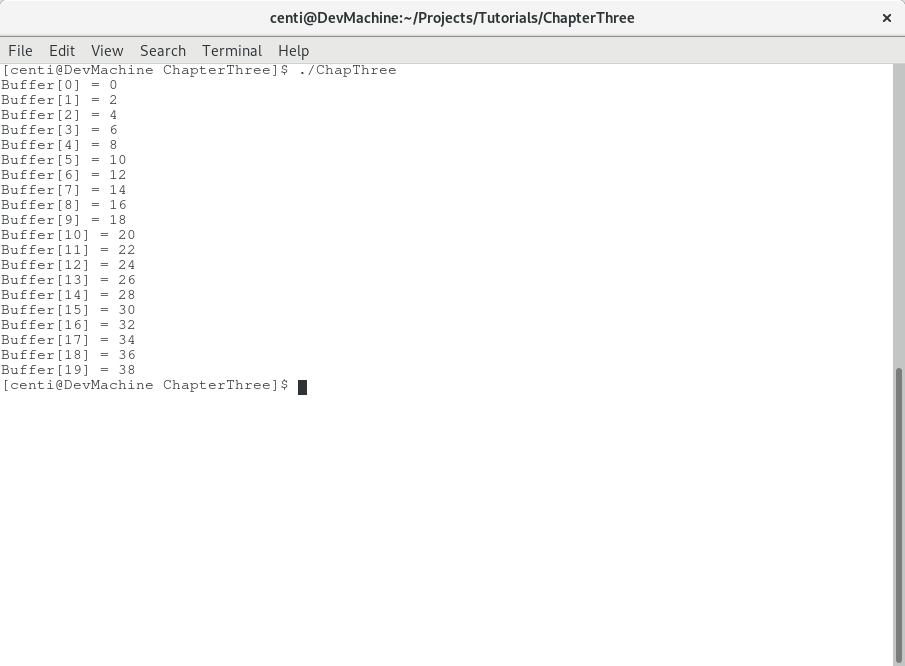
\includegraphics[width=\textwidth]{ChapThreeConsole}
\newpage
There are few things that may be confusing in the snippet above and why it is an acceptable practice in C:

\begin{enumerate}
	\item When you use malloc to allocate buffer, malloc keeps a record of how big the block of memory is so that it can be freed in later time, however you cannot and should not access that size information within malloc, keeping track of buffer size is your responsibility.
	
	\item When using malloc, you allocate the amount of data you would need by using sizeof keyword to determine how many bytes capacity you need in a buffer to cover that information and you can multiply that element size by the number of elements you want allocated for your program. In the snippet above, size of int32\_t type would resolves to 4 and then multiplied by 20, so we would have a buffer that have the capacity to hold 20 int32\_t elements.
	
	\item Malloc does not zero out the memory by default and in this specific case shown above, it's much more efficient since it's not necessary to zero out the memory since whatever memory/value stored in that allocated memory would be modified immediately after allocating. It however important that you need to zero out or assign a value to the memory otherwise when you attempt to read the said memory it would present an undefined behavior since you can't alway be sure the program will behave consistently when there are random value stored in the allocated memory and being processed by the program.
\end{enumerate}

Because of the fact behind malloc/free that LibC does store information about the pointer that is allocated with those functions, it discouraged to use different library or framework to free that memory, although most library and framework may likely use the same functions.
\newpage
\section{The Function Pointers}
Function pointers are a bit of a tongue twister, because the way it is defined in C can be confusing.

\lstinputlisting[style=customc, language=C]{codes/Chap3/Chap3Snippet4.c}

The snippet above is a declaration of function pointer for a function that returns a int32\_t after accepting two int32\_t parameters. It currently pointing at nothing and would cause segmentation fault when you attempt to call it, so you have to assign a function for it to be used.

One example of this use case is that we can dynamically modify the behavior of our program during runtime and essentially allow our program to switch logic at different points during program execution like so:
\lstinputlisting[style=customc, language=C]{codes/Chap3/Chap3Snippet5.c}
\newpage
It would produce an output as followed:

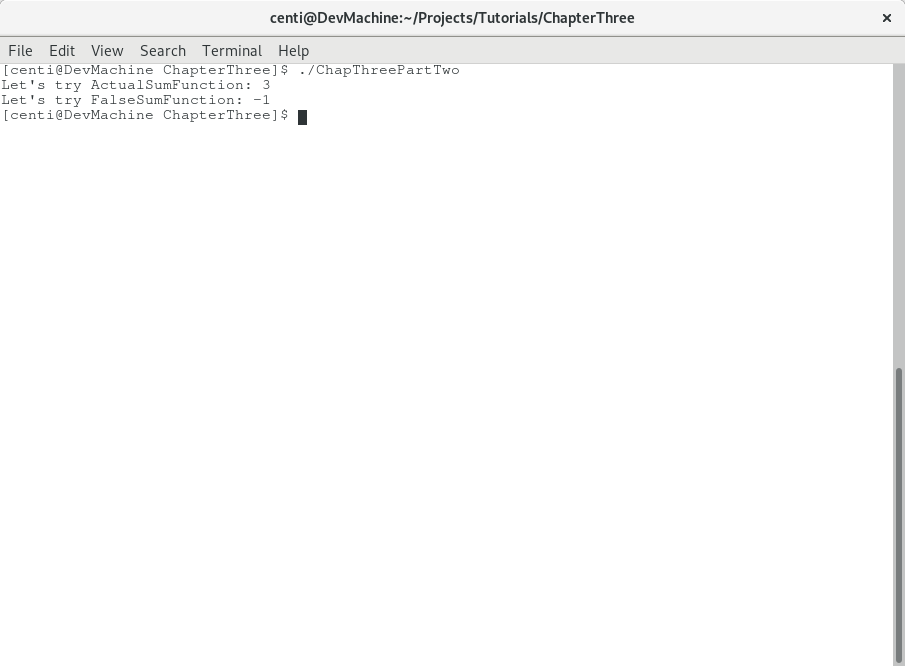
\includegraphics[width=\textwidth]{ChapThreeConsoleTwo}
\newpage
\section{C\# Counterpart}
C\# does support pointer in a similar fashion as C so long that the code blocks, methods, or types are defined with unsafe modifier. Those can be accomplished by using snippets below as a demonstration:
\lstinputlisting[style=customcs]{codes/Chap3/Chap3Snippet6.cs}
\lstinputlisting[style=customcs]{codes/Chap3/Chap3Snippet7.cs}
\lstinputlisting[style=customcs]{codes/Chap3/Chap3Snippet8.cs}

Though this is not required, you can use IntPtr and Marshal static class to accomplish everything of above.

When using \textbf{unsafe} modifier, compiler will throw an error unless you explicitly specify that you want to compile unsafe code. For CoreCLR, you can do so by adding the following into your csproj file inside the  <PropertyGroup> tags:

\lstinputlisting[style=customxml, language=XML]{codes/Chap3/Chap3Snippet9.xml}

Marshal static class from System.Runtime.InteropServices offer a variety of functions for marshaling pointers to usable data types and vice versa. You can also generate a function in runtime in CLR and pass it over to C program so that C program can use your newly created function during it's execution.

Passing a runtime generated function to C will be covered in Chapter 5.
